\documentclass[11pt]{article}

\usepackage{authblk} % for title page

\usepackage[margin=1in]{geometry} % to adjust margins

\usepackage{booktabs} % for pretty tables

\usepackage[labelfont=bf]{caption} % for pretty captions
\captionsetup[figure]{labelfont={bf},name={Fig.},labelsep=period} % Change formatting of figure caption start
\captionsetup{labelfont={bf},labelsep=period} % Change formatting of table caption start

\usepackage{lineno} % for line numbers

\usepackage{setspace} % for line spacing

% \usepackage[numbers]{natbib} % for bibliography
\usepackage{natbib} % for bibliography
\bibliographystyle{unsrtnat}

\usepackage{hyperref} % for internal links

\usepackage{pdflscape}

\usepackage{xr} % to reference supp mat
% \externaldocument{supp_mat}
% NOTE: if compiling from RStudio, need to make sure that the delete aux file option in Global Options is unchecked for this to work.

\usepackage{Sweave}
\begin{document}

\title{Data management group}
\author[1]{M. Bontrager}
\author[1]{E. Beyen}
\author[2]{E. Suglia}
\author[3]{J. Gremer} 
\author[3]{E. Elwood}
\author[2]{D. De La Pascua}
\author[4]{L. Leventhal}


\affil[1]{Still dreaming}
\affil[2]{Cat room-mate}
\affil[3]{Dog room-mate}
\affil[4]{Reunited with dog?}

\maketitle
\tableofcontents

\section{A section}
\label{why_latex}

LaTeX is a fancier typesetting program. It can do almost anything and is incredibly customizable.  It is open source and works similarly to Markdown: you write in a plain text file, then compile to the formatted version. I use it for my CV and for manuscripts. 
% Comments, other ideas, etc. can be interspersed with text.
It is especially preferred by people with a lot of equations in their work, because it formats them well. However, it has other features that are broadly useful: 

\begin{itemize}
\item{It formats references and bibliographies.}
\item{It is excellent for internal referencing. For example, when Figure 1 becomes Figure 2, those numbers change automatically (it can even do this with a separate supp mat file).}
\item{It imports figures from files so that each time you compile a document it will have the freshest version of your figures.}
\item{It makes pretty tables (they’re a bit of a pain to create but there are tricks in R).}
\item{For me, the process matches my flow when writing. There’s a source doc that is a mess, with notes, alternative phrasings of things, etc. and also a clean compiled version that I can read without seeing all the underlying chaos.}
\end{itemize}

\section{Another section}


I outlined some stuff about latex in Section \ref{why_latex}.


\subsection{What about references?}

You can cite references pretty easily, either paranthetically \citep{turesson1922species, clausen1948experimental} or in the text. For example, in \citet{savolainen2007gene}...

\subsection{What about equations?}

Equations can be written in line, for example, $\omega = \frac{xy + y^2}{V_S}$, or in blocks:

\begin{equation}
  \omega = \frac{xy + y^2}{V_S}.
\end{equation}

\subsection{What about figures?}

What if we include another figure? Well, they are numbered automatically and this new one is Figure \ref{height_leaf}.

One of the really nice things about latex is that you reference figure files which get pulled into your pdf. For example, Figure \ref{size} shows sizes for each population. 


\subsection{And tables?}

Tables are a bit of a pain to make, but in addition to typing them in manually, you can use R to convert any dataframe or csv file into a text file with latex formatting, which can then be pasted in to your manuscript. An example of a simple table is in Table \ref{studies_table}.

\clearpage

\begin{figure}
\centering
  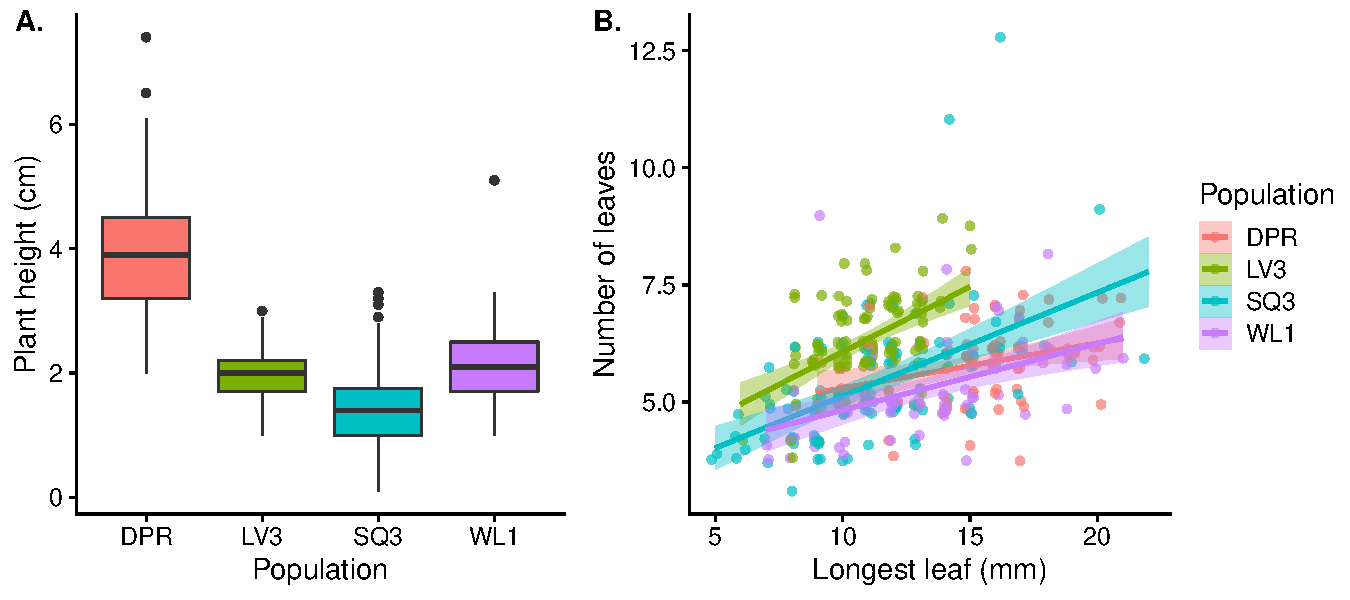
\includegraphics[width=\textwidth]{../plots/size_by_pop.pdf}
  \caption{A figure, which shows size by population in the vernalization experiment plants from the 10 week cohort of crossed plants.}
  \label{size}
\end{figure}

\begin{figure}
\centering
  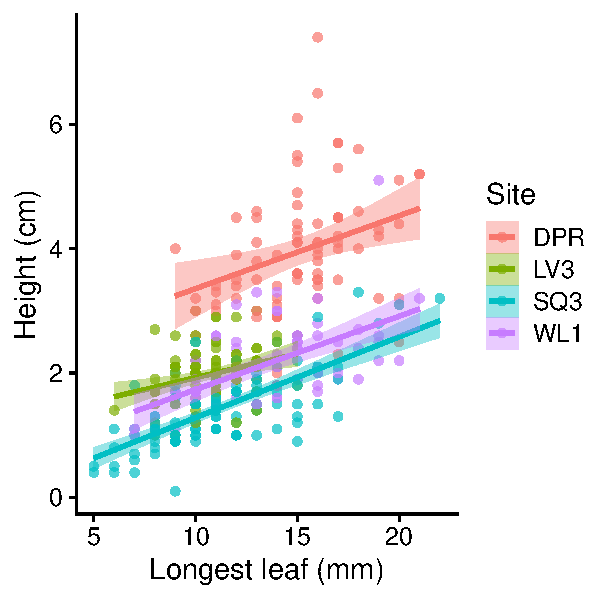
\includegraphics[width=9cm]{../plots/height_leaf.pdf}
  \caption{A figure, which shows the correlation between height and the length of the longest leaf. Each color is a different population.}
  \label{height_leaf}
\end{figure}


\clearpage

% \begin{center}
\begin{table}
\scriptsize
\caption{Studies included in our database. All studies were used in analyses of relative fitness, but only a subset of studies that included local populations in their design were included in our analyses of local adaptation. }
\begin{tabular}{lllcc}
\toprule
Study & Taxon   & Functional & Number    & Number      \\
      &         & group      & of sites  & of sources  \\
\midrule
Abdala-Roberts and Marquis 2007     & \textit{Chamaecrista fasciculata} & annual &  3 &   3  \\
Adler et al.\ 2016                      & \textit{Gelsemium sempervirens} & herb.\ per. &  2 &   9   \\
Afkhami et al.\ 2014                 & \textit{Bromus laevipes} & herb.\ per. & 10 &   6  \\
\r{A}gren and Schemske 2012         & \textit{Arabidopsis thaliana} & annual &  2 &   2  \\
Alexander 2010                & \textit{Lactuca serriola} & annual &  5 &  10   \\
Alexander et al.\ 2012                  & \textit{Plantago lanceolata} & herb.\ per. &  4 &  15  \\
Andersen et al.\ 2008         & \textit{Abies guatemalensis} & wood.\ per. &  2 &   9  \\
Anderson et al.\ 2015                 & \textit{Boechera stricta} & herb.\ per. &  3 &  50  \\
\bottomrule
\end{tabular}
\label{studies_table}
\end{table}
% \end{center}




\bibliography{refs}

\end{document}
